\documentclass[11]{article}


\usepackage{wrapfig}
\usepackage{makecell}
\usepackage{float}
\usepackage{graphicx}
\graphicspath{{./imgs/}}
\usepackage[margin = 1in]{geometry}
\usepackage{indentfirst}

\begin{document}

\begin{titlepage}
	\begin{center}	
		
\includegraphics[width = 5cm,height = 1.5cm]{uws_logo.png}\\[5cm]
	
{ \huge \bfseries %
		How can online learning platforms use mobile technology to expand their market and generate new revenue?\\ \Large 
}
	\vspace{2cm}
	
	{\huge
		% Mobile Business Technology \& Design
	}

	\vspace{2cm}			
			
		\begin{flushright}
				\large Student:\\
				Marius-Lucian Olariu\\[1cm]
		\end{flushright}
		
	
		\begin{flushleft}
			 \large
				Module coordinator: \\
				Mark Stansfield \\[1cm]
		\end{flushleft}
		
	\vspace{2cm}	
	
		
		\vfill
		
		{\large {Paisley \\ 2019}}
		\end{center}
\end{titlepage}

\newpage

\tableofcontents

\listoffigures

\listoftables

\newpage
\section{Introduction}(800 words)\\

		Electronic Learning (E-learning) is instruction delivered on a digital device that is intended to support learning (Clark and Mayer, 2016). Most of the people would think of digital devices as being personal computers, smartphones or tablets but  in its primary form the e-learning started with televison/radio broadcasting  educational programs or accessing information through mainframe computers in the 1950s. Nowdays, this field comprises Web-based learning, Webinars, Virtual Classoom (online portals - video conferencing between learners and teachers) or Mobile Learning . E-learning  aids business to deliver training to their employees and even degrees from accredited universities around the world or invididuals to acquire knowledge and skills.\\

		\indent
		New opportunities arose for educational institutions and private companies, namely to use digital devices to provide \textit{Distance Learning}.
		Distance Learning has been around for more than 100 years now through the help of televesion and radio that  broadcasted occasionally courses. However, they were not that popular; all this has changed with the rise of Internet and the multimedia systems that made courses available all the time, no matter the location of the learner. In other words, an evolution occured in education. Nowadays, there are a lot of online learning platforms like \textit{Coursera}, \textit{edX} or \textit{XuetangX} that seem so appealing compared to traditional education due to low-cost, accessibility and flexibility. All the above mentioned online platforms provide \textbf{M}assive \textbf{O}pen \textbf{O}nline \textbf{C}ourses (MOOCs) that represent a postindustrial model of teaching and have great success in an industry with 101 milion learners online, 900+ universities involved and around 11 thousand courses (By The Numbers: Moocs In 2018 — Class Central, 2018) . Online courses are tailored for different levels of understanding of a subject (e.g. basic, intermediate or advanced) and aim to help solving the problem of  access to education world-wide. Moreover, the learner has the option to  choose from a wide range of courses teaching a particular subject (e.g. machine learning) often on the same platform (e.g. different institutions publish they course variant on Coursera), whereas when studying on-site the learner (or student, in this case) does not have this possibility. Despite of the mentioned benefits that these online platforms bring, all of them face one big issue, namely the credibility of the courses they provide. In order to solve this problem some of the online platforms accept courses created only by accredited universities and individuals, though, this is not a practice that all the online platforms follow. As a result, addressing this problem of quality is very important for their credibility and mass adoption by the public.\\
Next, in general the online courses are, as mentioned above, tailored on different levels (e.g. basic, intermediate, advanced), whereas most of the times there is a need to adapt the course to each individual learner as was demonstrated by Bloom (1984). In face-to-face education a teacher can adapt the content of the course to better suit the vast majority of a class or provide extra help for some individuals. However, over time this situation can change since it is easy to embbed new research findings into the online platform to best enable learning.\\
Lastly,  on-site learning has an advantage over online/distance learning because it provides on-campus opportunities to socialize and build up a network. Along this line of thinking, traditional institutions might survive to the Internet disruption because they do not provide only information to learners (Wessel and Christensen, 2012). \\
\begin{figure}[H]
	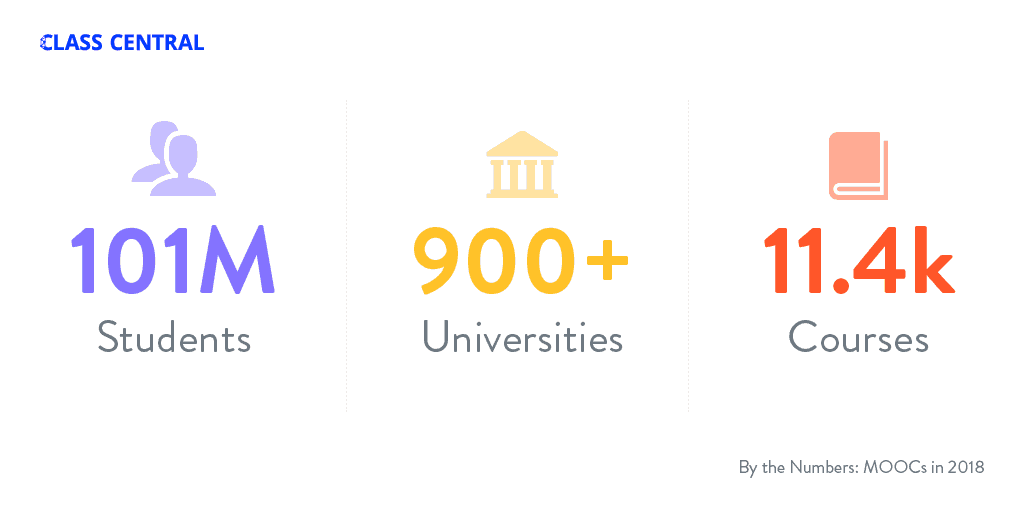
\includegraphics[scale=0.45]{stats.png}
	\caption{Overview of the online learning industry (By The Numbers: MOOCs in 2018, 2018)}	
\end{figure}
\indent
	Until this point we discussed about online learning that is performed through the help of websites but in recent years this field has shifted towards the use of mobile technology.  Mobile technologies are a part of our daily life and we are deeply reliant on them; Ray Kurzweil, an American inventor and futurist, even sees them as "brain extenders". There has been coined a term for learning using mobile technology, namely \textit{Mobile Learning} (M-Learning), which essentially is a type of e-learning that refers to the aquisition of knowledge and skills by using mobile technologies such as smartphones, audio players or tablets. However, the most popular technology is the smartphone due to the fact that it provides other services like Internet browsing, photography, GPS, and others. Online learning through the help of online portals brings flexibility compared to traditional teaching, however, porting this online portals to mobile through native mobile applications takes flexibility a step further since the mobile device can be carried everywhere by the learner. According to Thornton and Houser (2005) a mobile learning environment increase the transfer of knowledge and feedback. Nonetheless, some suggest that mobile learning aims to improve the learning experience but should not be used as the primary method to provide a course (Wang et al. 2009). M-Learning has its own challenges which are summarized in Table~\ref{mLearChall}.


\begin{table}[H]
	\centering
	\caption{Challenges faced by M-Learning}
	\label{mLearChall}
	\begin{tabular}{|c|c|}
		\hline
		\textbf{ Challenge } & \textbf{Note}  \\
		\hline
		Lack of motivation & \makecell { Even if a company buys courses for employees they might pass\\ them by searching answers to tests on forums\\ and not by engaging with the course material}  \\	
		\hline
		Security of user & \makecell{The device needs to be carried and the individual\\ is not fully aware of what is happening around him}  \\	
		\hline
		Self-directed learning & \makecell{General concern in online learning, some of users\\ are autodidacts or advanced learners and can find\\ our own route in e-environment while others not}  \\	
		\hline
		Absence of social interaction & \makecell{Peer mentoring plays an important role in traditional education\\ and it is hard to create this in an online environment}\\
		\hline
	\end{tabular}
\end{table}

\newpage
\section{Analysis of mobile technologies in online learning}(1400 words)
	All the online learning platforms have developed their mobile applications in order to increase the number of learners they can reach. In order to teach a course they make use of videos and subtitles, quizzes, projects and presentation slides. Also the content can be downloaded so offline access of it is possible. 

	\subsection{Sources of monetization}

	
\section{Case studies: Coursera and edX}(1400 words)

	\subsection{Coursera}
	Coursera is an online learning platform that provides courses, specializations and online degrees (see Figure~\ref{courseraLogo}). It was founded in 2012 by two computer scientist from Standford University, namely, Andrew Ng and Daphne Koller. The founders were inspired to create this platform because one year before, in 2011, they have provided online courses. Up to this date the company has managed to raise \$210 millions from different organizations. Currently this company is leading the field from the perspective of registered users, having more than double compared to the next competitor (see Table~\ref{top5}). Things are good when it comes to revenue as well, Coursera's revenue for 2018 was estimated to be \$140 million and was listed in The Next-Bilion Dollar Startups (2018) by Forbes.

\begin{wrapfigure}{r}{10cm}

	\begin{center}
		
\includegraphics[width = 0.5\textwidth]{courseraLogo.png}
	\end{center}
	
	\caption{Coursera logo}
	\label{courseraLogo}

\end{wrapfigure}

\begin{table}[H]
	\centering
	\begin{tabular}{|c|c|c|}
		\hline
		\textbf{\#} & \textbf{Online Provider} & \textbf{\# of users} \\
		\hline
		1 & Coursera & 37 million \\
		\hline
		2 & edX      & 18 million \\
		\hline
		3 & XuetangX & 14 million \\
		\hline
		4 & Udacity & 10 million \\
		\hline
		5 & FutureLearn & 8.7 million \\
		\hline
	\end{tabular}

	\caption{Top 5 online platforms based on number of registered user (By The Numbers: MOOCs in 2018, 2018)}
	\label{top5}

\end{table}

   	\paragraph{Monetization\\}
	The source of revenue for Coursera has switched from charging per course to charge for getting certification for completion of a course, nowadays, auditing a course is free of charge. Other sources of revenue are specializations, online degrees and corporate training. Specializations are groups of courses aimed to master a specific skill (e.g. Deep Learning), they take between 4-6 months to complete and are priced per month (price range: \$39 - \$79). Online degrees are just like traditional degrees a form of education which typically takes between 1-3 years and are taught entirely online in our case. At the end, the learner has an degree from accredited university. However, these online degrees do not stick to the initial ideal of MOOCs of providing knowledge and skills at an affordable price since they are just a bit cheaper than studying on-campus, they cost between \$15 000 and \$25 000. Like in the traditional case to enroll for an Online Degree the learner has to go through an admission process. To name but a few universities who provide Online Degrees on Coursera: University of London, Arizona State University, HEC Paris or Imperial College London. talk about coursera for business\\  

	-> Eighty-nine percent of Coursera learners are over the age of 22. "life-long learners" -> professionals who look for career growth. Lifelong career learning driven by necessity of constantly adapting to the changing job market.
	-> own proprietary credentials created for professionals learners. They submited a list of possible specializations, universitites would bid on them (rank them) and the top specializations would receive a \$100 000 to be created.
	not enough to create specializations, the available free options shrunk. Started to target companies who have money allocated for employees training, bigger market than direct to consumer. => Coursera for Business product
	->earning academic credit for MOOCS
	-> 3 monetization sources: direct to consumer, corporate training and online degrees.
	\subsection{edX}

\newpage
\section{References}
By The Numbers: MOOCs In 2018. (2018) Available: https://www.class-central.com/report/mooc-stats-2018/ [Accessed: 27 February 2019]\\

Bloom, B.S., 1984. The 2 sigma problem: The search for methods of group instruction as effective as one-to-one tutoring. Educational researcher, 13(6), pp.4-16. \\

Wang, Y.S., Wu, M.C. and Wang, H.Y., 2009. Investigating the determinants and age and gender differences in the acceptance of mobile learning. British journal of educational technology, 40(1), pp.92-118.\\

Hamidi, H. and Chavoshi, A., 2018. Analysis of the essential factors for the adoption of mobile learning in higher education: A case study of students of the University of Technology. Telematics and Informatics, 35(4), pp.1053-1070.\\

Mazoué, J.G., 2012. The deconstructed campus. Journal of Computing in Higher Education, 24(2), pp.74-95.\\

The Next Billion-Dollar Startups (2018) Available: https://www.forbes.com/next-billion-dollar-startups/\#246a9dbe4441 [Accessed: 28 February 2019].\\

Thornton, P. and Houser, C., 2005. Using mobile phones in English education in Japan. Journal of computer assisted learning, 21(3), pp.217-228.\\

Wang, Y.S., Wu, M.C. and Wang, H.Y., 2009. Investigating the determinants and age and gender differences in the acceptance of mobile learning. British journal of educational technology, 40(1), pp.92-118.\\

Wessel, M. and Christensen, C.M., 2012. Surviving disruption. Harvard Business Review, 90(12), pp.56-64.\\

\end{document}

